\documentclass{article}
\usepackage[a3paper,landscape]{geometry}
\usepackage[brazil]{babel}
\usepackage{graphicx}
\usepackage[utf8]{inputenc}
\usepackage{sectsty}
\usepackage{longtable}
\usepackage{subfigure}
\usepackage{adjustbox}
\usepackage[table]{xcolor}    % loads also colortbl
\title{ Teoria da Computação 2024/2}
\date{}
\author{ prof. Daniel Saad}
\allsectionsfont{\centering}
    
\begin{document} \maketitle
    \rowcolors{2}{white}{gray!25}
    \begin{longtable}{|l|c|c|c|c|c|}
    \hline
Matrícula & Prova 1 & Prova 2 & Prova 3 & Prova Substitutiva & Nota Final\\\hline \endhead   
141057600003 & 2.0 & 3.0 & - & - & 1.7\\\hline
151057600064 & - & - & - & - & 0.0\\\hline
161057600019 & - & - & - & - & 0.0\\\hline
161057600065 & - & - & - & - & 0.0\\\hline
181057600001 & - & - & - & - & 0.0\\\hline
191057600007 & 10.0 & 6.2 & 5.1 & - & 7.1\\\hline
191057600009 & 9.0 & 5.5 & 5.0 & - & 6.5\\\hline
191057600048 & 2.4 & 4.0 & - & - & 2.2\\\hline
191057600051 & 8.7 & 3.4 & 8.6 & - & 6.9\\\hline
201057600003 & 10.0 & 7.7 & 4.8 & - & 7.5\\\hline
201057600023 & - & - & - & - & 0.0\\\hline
201057600034 & - & - & - & - & 0.0\\\hline
211057600002 & - & - & - & - & 0.0\\\hline
211057600015 & - & - & - & - & 0.0\\\hline
211057600034 & - & - & - & - & 0.0\\\hline
211057600049 & 7.6 & 7.1 & 4.7 & - & 6.5\\\hline
211057600056 & 5.5 & - & - & - & 1.9\\\hline
212057600001 & 1.7 & - & 5.0 & 1.4 & 2.7\\\hline
221057600010 & 9.4 & 8.1 & 7.4 & - & 8.3\\\hline
221057600014 & 10.0 & 6.9 & 7.0 & - & 8.0\\\hline
221057600015 & 2.7 & 4.5 & 7.4 & - & 6.0\\\hline
221057600020 & 1.7 & - & - & - & 0.6\\\hline
221057600022 & 9.3 & 9.6 & 5.4 & - & 8.1\\\hline
221057600023 & 10.0 & - & - & - & 3.4\\\hline
221057600025 & 10.0 & 6.8 & 3.4 & - & 6.8\\\hline
221057600029 & 10.0 & 8.8 & 8.6 & - & 9.2\\\hline
221057600033 & 2.0 & 1.8 & - & - & 1.3\\\hline
221057600035 & 9.7 & 4.8 & 5.4 & - & 6.7\\\hline
221057600037 & - & - & - & - & 0.0\\\hline
221057600048 & 4.8 & 1.6 & 2.4 & - & 3.0\\\hline
221057600055 & 9.4 & 10.0 & 8.6 & - & 9.4\\\hline
221057600061 & 10.0 & 5.2 & 8.6 & - & 8.0\\\hline
221057600066 & 5.9 & 5.0 & 4.7 & - & 6.0\\\hline
\end{longtable}
\begin{figure}[h!]
\centering\begin{subfigure}
        \centering
        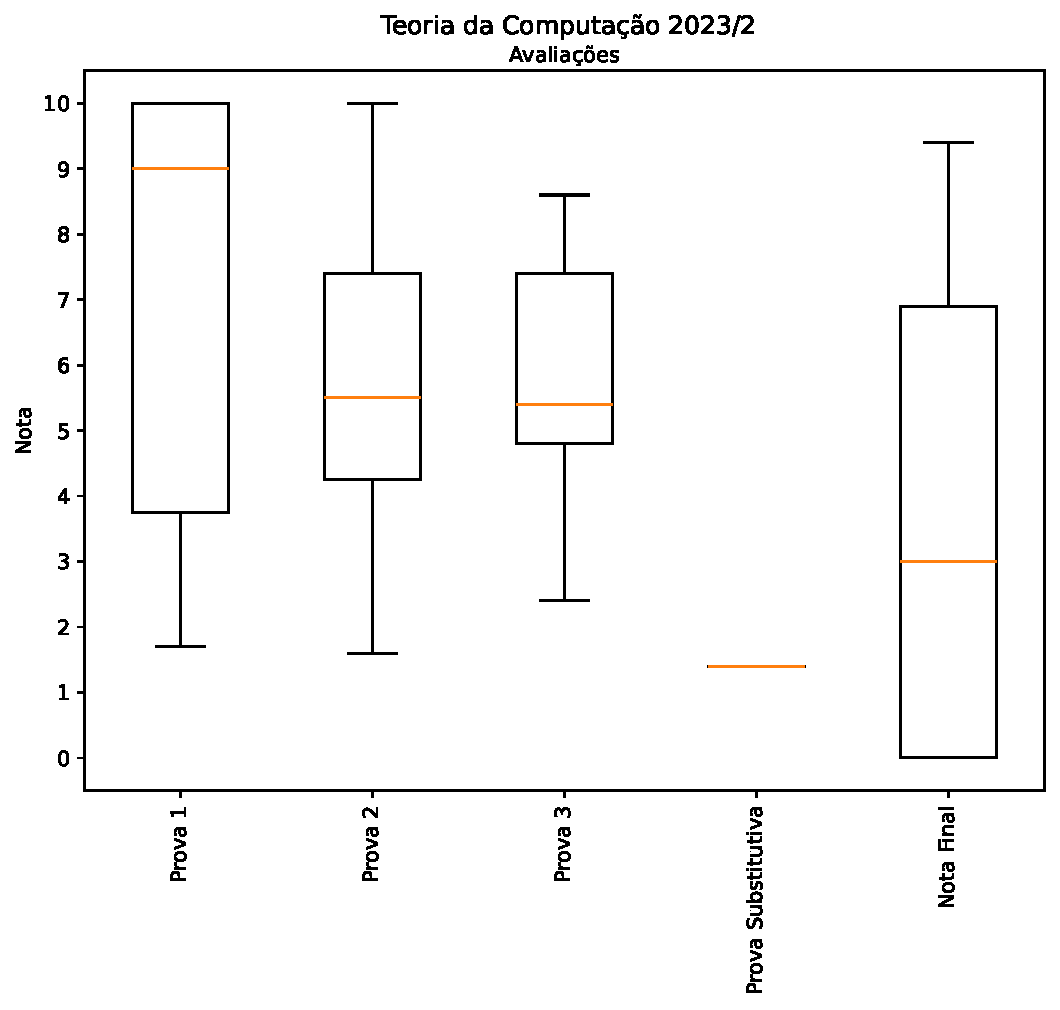
\includegraphics[width=.8\textwidth]{/home/danielsaad/git/ifb/disciplinas/teoria-da-computacao/assets/boxplot.pdf}
    \end{subfigure}\end{figure}\end{document}
